%!TEX root = pfe-book4.tex
%!TEX TS-program = pdflatex
%!TEX encoding = UTF-8 Unicode


\cleardoublepage
%\mainmatter
\chapter{Hard Electromagnetic Radiation}
\label{ch-03}

\section{The Discovery of X-Rays}

\emph{$X$-rays} is the term used for radiation occupying a portion of the electromagnetic spectrum approximately from several tens of nanometres to 0.01 nanometre. The still harder (that is, having still shorter wavelengths) rays are called \emph{gamma rays}.

As we have already mentioned, the names for the various portions of the electromagnetic spectrum are rath­er conventional. The term designating each portion of the spectrum has less to do with the wavelength than with the nature of the source of radiation. Most frequent­ly, the term ``$X$-rays'' is used for radiation that occurs when a flux of electrons encounters an obstacle.

Wilhelm Conrad Roentgen (1845-1923) discovered this kind of radiation on November 8, 1895. During those years, many physicists around the world were studying fluxes of electrons arising in evacuated glass tubes (illus­trations of these are given in Figure 2.6 of the third book of this series). Two electrodes were soldered into a vessel and a high voltage applied. The fact that some kind of rays were emitted from the cathode of such a tube had been suspected for quite some time. At the very beginning of the $19^{\textrm{th}}$ century a number of researchers observed flashes inside the tube, a fluorescence of the glass. Through the experiments of the German physicist Johann Wilhelm Hittorf (1824-1914) and the English chemist and physicist William Crookes (1832-1919) it was demonstrated that these were rays, in the path of which an obstacle had been placed. All textbooks included a pho­tograph of the \emph{Crookes tube} with a cross which he made in 1878, nine years after Hittorf. The cross threw a definite shadow onto the glass. This elegant experiment proves that some kind of rays emanate from the cathode and move in straight lines. When the rays fall on the glass, it glows and a thin layer of metal absorbs the radiation.

The fact that cathode rays are a flux of electrons was proved by Sir Joseph John Thomson (1856-1940) in 1897. By a method discussed in the third book of this series he was able to determine the ratio of the charge to the mass of the electron. Another 10 to 15 years passed and it became clear that the electron is a minute particle of electricity.

But we are going astray. What interests us now is the discovery made by Roentgen. However, our brief digres­sion was made to emphasize the fact that Roentgen's discovery preceded an understanding of the nature of the rays emitted by the cathode. Actually, it was precisely because of a lack of understanding that Roentgen was investigating a variety of tubes with different locations of electrodes and different forms of glass envelope.

The events of the evening of November 8, 1895 are perfectly well known. Roentgen placed a piece of black cloth over the tube, turned off the light in the room, and was about to go home with the light switch left on. Then he glanced at the instrument he was working with and noticed that the screen covered with barium platino-cyanide (which is capable of fluorescing) next to the tube was glowing. Roentgen returned, threw the switch, and the fluorescence ceased. He turned on the switch and the screen began to glow anew. Roentgen knew that in the tube of the design he was working with, cathode rays could not pass through the protective covering thrown over the tube and then through a big layer of air as well. That could only mean one thing -- a new hitherto unknown kind of radiation.

Roentgen first reported his discovery at the end of the year. During this interval he had made such a thorough study of the properties of the new rays that up until the discovery of the diffraction of $X$-rays by a crys­tal (1912) -- we will come to that soon -- nothing new about the $X$-rays was unearthed. The name $X$-rays was given by Roentgen himself, but in some countries the radia­tion is termed Roentgen rays.

\begin{figure}[!ht]
\centering

\includegraphics[width=\textwidth]{figures/fig-03-01.pdf}
\caption{$X$-rays penetrate muscles and can show the skeleton.}
\label{fig-3.1}
\end{figure}


The most remarkable property of $X$-rays is the property that Roentgen studied and illustrated from the very start: their ability to pass through materials that are opaque to light. (\figr{fig-3.1} is a reminder of the many caricatures that appeared two or three months after Roentgen's first publication.)

The penetrating power of $X$-rays was a boon to medi­cine. It also became possible to detect imperfections in industrial goods. The amazing results of roentgenography stem from the fact that materials of different density absorb $X$-rays to different degrees. The lighter the atoms of the material the less the rays are absorbed.

It was also soon found that the penetrating power of the rays increased with increasing voltage in the tube. Voltages ordinarily used in $X$-ray equipment are between several tens and several hundreds of kilovolts.

Research into the properties of $X$-rays elicited the fact that they are caused by retardation of electron fluxes due to an obstacle. It is curious thing to recall that for quite a long time Roentgen tubes were manufactured with three electrodes. An ``anticathode'' was fitted opposite the cathode to receive the impinging electrons. The anode was placed to one side. A few years later it became clear that that was a needless complication and today two electrodes are used. A flux of electrons impinges on the anode, the surface of which is beveled. Then the flux of $X$-rays is directed where needed. If the surface of the anode meets the electron flux at right angles, the rays go off the anode in all directions and we lose a certain amount of intensity.

The use of $X$-rays created a revolution in industry and medicine. $X$ray technology today is a highly refined field. By varying the position of an object relative to the $X$-ray tube, we can obtain several pictures, thus enabling us to establish the exact position of a defect not only in projection but also its depth within the ma­terial.

Depending on the materials or tissues being investigat­ed, use is made of hard (more penetrating) radiation or soft radiation. The main purpose is to attain a contrast so as to see the defect, which may differ in density only slightly from the main material.

The \emph{law of absorption of $X$-rays}, like the law of absorp­tion of any other radiation, is quite obvious. What in­terests us is how the intensity of radiation (recall that intensity is energy per unit time and unit area) changes after passing through a plate of thickness $d$. Since this book is for the reader who is not acquainted with integral calculus, I will confine myself to the statement of the law for radiation passing through thin plates. ``Thin'' stands for the intensity falling off very slightly, say about 1\%. In that case the law is simple: the portion of absorbed radiation is directly proportional to the thickness of the plate. If the intensity diminishes from a value $I_{0}$ to a value $I$, then this simple rule can be written thus:
\begin{equation*}%
\frac{I - I_{0}}{I} = \mu d
\end{equation*}
The proportionality factor $\mu$ is called the \emph{absorption coefficient}.

Here is a simple question I have posed at examinations: In what units is the absorption coefficient measured? This is an easy question. The units of measurement have to be the same on both sides of the equation. That's clear. You can't say that 10 kilograms is more than 5 me­tres. The only comparisons can be between kilograms and kilograms, amperes and amperes, ergs and ergs. And so the units are the same on both sides of the equation.

Now, in the left-hand member of this equation we have a dimensionless number. By saying that the portion of absorbed radiation is equal to 1/30 or 0.08, we have said all there is to say. The units of measurement cancel out when intensity is divided by intensity. And that means that the quantity on the right must be non-dimensional. Since thickness is measured in centimetres (or other units of length), the absorption coefficient is measured in inverse centimetres, that is, \si{\per\centi\meter}.

Suppose a ray passes through a \SI{10}{\centi\meter} thick plate and loses 1\% of its intensity. The left-hand side of the equa­tion is equal to 1/100. This means the absorption coeffic­ient here is equal to \SI{0.001}{\per\centi\meter}. Now if the radiation is soft and loses one percent of its energy when passing through a foil one micrometre (\SI{0.0001}{\centi\meter}) in thickness, then the absorption coefficient will be \SI{100}{\per\centi\meter}.

Physicists do not have a good theory for establishing a formula for the absorption coefficient. I can only say that the absorption coefficient is roughly proportional to the cube of the wavelength of $X$ radiation and to the cube of the atomic number of the substance through which the radiation is passing.

Since the wavelengths of $X$-rays are extremely short, the frequencies of the electromagnetic waves are high. This means that a quantum of $X$-rays, $h\nu$, carries a tremendous energy. This energy is only sufficient for chemical reactions leading to blackening of the emulsion of a photographic plate and the phosphorescence of screens (even light waves can do that), but there is even more than enough to break up molecules. In other words, $X$-rays ionize air and other media through which they pass.
Now a few words about gamma rays. This term applies to the short-wave radiation that originates in radioactive decay. Gamma rays are emitted by naturally radioactive substances and are produced by artificial elements. A nuclear reactor generates gamma radiation of course. Very hard (high-energy) gamma rays are produced in the ex­plosion of an atomic bomb.

Since gamma rays can have a very short wavelength, their absorption coefficient can be very small. For instance, the gamma rays that are emitted in the disintegration of radioactive cobalt are capable of passing through tens of centimetres of steel.
Substantial doses of short-wave electromagnetic radia­tion (such that is capable of disrupting molecules) are very dangerous to any living organism. Therefore protec­tion is needed when dealing with $X$-rays and gamma rays. Ordinarily it is in the form of lead. The walls of $X$-ray rooms are covered with a special coating containing barium salts.

Gamma rays, like $X$-rays, can be used for radioscopy. Usually use is made of the gamma rays of radioactive substances which are the ``ashes'' of nuclear fuel. Their advantage over $X$-rays is the extreme penetrating power, but most important of all is the possibility of using, as the source of radiation, a small ampoule that can be fitted into places that are inaccessible to an $X$-ray tube.

\section{X-ray Diffraction Analysis}

In 1912 Roentgen was head of the chair of physics at the University of Munich. Problems dealing with the nature of $X$-rays were constantly being discussed. I must say that Roentgen, who was an experimental physicist himself, had much respect for theory. There were a good many talented theoretical physicists at the chair of physics at the University of Munich that were cudgelling their brains over the nature of these new $X$-rays.

And of course attempts were made to investigate the nature of the $X$-rays by passing them through a diffrac­tion grating. Using a diffraction grating, one can prove quite definitely the wave nature of light and also obtain exact determinations of the wavelength of one or another type of radiation.

One way of making such a grating is to rule fine scratches on a glass plate coated with aluminium; this is done with a cutting tool made of ivory. The lines thus cut must be strictly equally spaced. A good grating must have a small period and a large number of lines. Up to hundreds of thousands have been ruled and over a thou­sand per millimetre.

With the help of a lens, a strong point source of light can produce a parallel beam of light that falls on the grating at right angles. The rays emerge from each aper­ture and proceed in all directions (in other words, each aperture becomes the source of a spherical wave). But only in certain directions will the waves from all apertures be in-phase. For reinforcement, it is necessary that the path difference be equal to an integral number of wavelengths. Strong rays will go in directions at an angle a that obey the condition 
\begin{equation*}%
a \sin \alpha = n \lambda
\end{equation*}
where $n$ is an integer and $a$ is the distance between slits. The reader can easily derive this formula without our help. The whole number $n$ is termed the \emph{order of the spec­trum}. If monochromatic light is incident on the grating, we obtain, in the focal plane of the eyepiece, several lines separated by dark intervals. If the light consists of waves of different wavelength, the grating will produce several spectra: of first, second, etc. orders. Each suc­ceeding spectrum will be more extended than the pre­ceding spectrum.

Since the wavelength of the light is of the same order as the distance between the slits, diffraction gratings disperse light (and not only visible light but also ultraviolet radiation and, best of all, infrared radiation) into spectra. These instruments make it possible to carry out a detailed spectral analysis of the radiation.

But in relation to $X$-rays, diffraction gratings behaved like a system of open doors. $X$-rays passed through them without deviating. It could be suspected that $X$-rays are a flux of particles. But, on the other hand, there was every reason to think that this $X$ radiation is the same electromagnetic field as light, only with the wavelength $\lambda$ much shorter. True enough, suppose the wavelength is very short. If that is so, then, according to the diffraction equation, all $n$ rays proceeding at diffraction angles a from the line optical grating $a \sin \alpha =n \lambda$ will practically merge and no diffraction will be apparent. But to make a diffraction grating with slits separated by a distance $a$ equal to millionths of a micrometre is out of the ques­tion. So what have we?

A young German physicist Max von Laue (1879-1960) was sure that $X$-rays are a type of electromagnetic radia­tion. His acquaintance was a crystallographer who was convinced that a crystal is a three-dimensional lattice of atoms. In one of their numerous talks on scientific topics, Laue got the idea of correlating his view of the nature of $X$-rays with the concept of a crystal as a lattice. Laue's idea was this: suppose the distances between the atoms of a crystal and the wavelength of $X$-rays were quantities of the same order.

Can a three-dimensional lattice take the place of a line grating of slits? It was not obvious at all, but Laue decided to try it. The first experiment was simplicity itself. A beam of $X$-rays was diaphragmed. A large crystal was placed in the path of the rays, and next to the crystal a photographic plate. True, it was not at all clear where to put the plate since the crystal was not a line lattice. The first attempts were thus failures. But soon, due to a mistake, they got the plate in the proper position.

This accidental mistake did not play any special role in the discovery because Laue was also working on the theory of the phenomenon besides trying to detect it. He was soon able to extend the theory of the line dif­fraction grating to the three-dimensional case. From the theory it followed that diffracted rays would appear only in the case of certain orientations of the crystal with respect to the incident rays. From the theory it also fol­lowed that the most intensive rays were those deflected
at small angles. And from this it was evident that the photographic plate had to be positioned behind the crystal perpendicular to the incident rays.

Among the first researchers to notice this discovery were the Braggs, the father Sir William Henry (1862-1942) and his son Sir William Lawrence (1890-1971), English physicists. They repeated Laue's experiment, provided a very simple and pictorial interpretation and also demonstrated many simple instances in which Laue's discovery could be used as a method for studying the atomic structure of substances.

Let us take a brief look at \emph{$X$\!--ray diffraction analysis} and also examine the path by which we can determine the structure of a crystal, that is, measure the distances between atoms with an accuracy of up to one hundredth of an angstrom and give a picture of the spatial arrange­ment of atoms in a molecule, and also determine the nature of the packing of molecules in a crystal.

Suppose a crystal is set in a special holder and rotates on an axis. The $X$-ray falls at right angles to the axis of rotation. What happens? Let us examine the diffraction phenomena that take place when an $X$-ray is incident on the crystal so that a lattice point is regarded as the scattering centre.

The Braggs (father and son) demonstrated that the scattering of $X$-rays by lattice points is equivalent to a curious kind of selective (that is, taking place only for certain discrete values of the angle) reflection of rays from a system of nodal planes, into which the lattice may be partitioned.

Suppose a ray, which is an electromagnetic wave of a definite length, falls on a crystal at some angle. This angle will differ for different systems of planes. We have every right to assume that any atomic plane will reflect the $X$-ray in accord with the law: the angle of incidence equals the angle of reflection. But there is essential dif­ference from optical rays. Unlike light, $X$ radiation pen­etrates deep into a crystal. This means that the reflec­tion of the ray will occur not from the external surface but from all atomic planes.

\begin{figure}[!ht]
\centering
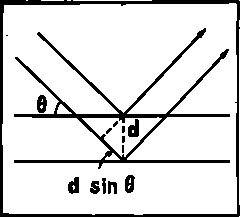
\includegraphics[width=0.4\textwidth]{figures/fig-03-02.pdf}
\caption{Rays reflected from a crystal with a path difference of $2d \sin \theta$.}
\label{fig-3.2}
\end{figure}

Let us consider one such system characterized by the interplanar spacing $d$. Each of them will ``reflect'' an incident ray at one and the same angle $\theta$. These reflected rays must interfere, and a strong secondary ray will arise only if the rays reflected from all planes of the family are in the same phase. In other words, the path difference between the rays must be equal to a whole number of wavelengths.

\figr{fig-3.2} depicts a geometric construction from which it follows that the path difference between adjacent reflected rays is equal to $2d \sin \theta$. Hence the condition of diffraction will be of the form
\begin{equation*}%
2d \sin \theta = n \lambda,
\end{equation*}
The Russian crystallographer G. V. Vulf arrived at this formula at the same time as the Braggs and so it is called the \emph{Bragg-Vulf} equation (also known as \emph{Bragg's law} or \emph{Bragg's equation}).

A crystal can be partitioned into systems of planes in numberless ways. But only a certain system becomes effective for reflection: that in which the interplanar spacing and orientation with respect to the incident ray are such that Bragg's equation is obeyed.

Obviously, if the ray is monochromatic (that is, the electromagnetic wave has a definite length), then reflec­tion may not occur in the case of an arbitrary position of the crystal with respect to the ray. However, by ro­tating the crystal we can bring different systems of planes into the reflecting position in turn. This appeared to be the most suitable way for practical work.

As for Laue's experiment, its success stemmed from the fact that the radiation incident on the crystal was the ``white spectrum'' of $X$-rays, that is, a flux of waves whose lengths are continuously distributed over a certain interval (see below). Therefore, although the crystal was fixed in Laue's experiment, different systems of planes appeared in the ``reflecting'' position for waves of different length.

At the present time, $X$-ray diffraction analysis is completely automatic. A small crystal (0.1 to 1 mm) is fixed in a special holder, which can turn the crystal according to a specified programme, bringing into the reflecting position all its system of planes one after the other. Every reflecting plane (we'll use that word so as not to repeat ``system'' all the time) is characterized, first, by its interplanar spacing, second, by the angles which it forms with the axes of an elementary cell of the crystal (lengths of the edges and the angles between the edges of the cell are measured first of all and automatically) and, third, by the intensity of the reflected ray.

The more atoms a molecule contains the greater (na­turally) the dimensions of the elementary cell. This in­ creased complexity brings with it a greater volume of information. The point is that the larger the cell the greater the number of reflecting planes. The number of measured reflections can range from several tens to sev­eral thousands.

We promised a brief survey of the idea underlying $X$-ray diffraction analysis. Let us first turn the problem around. Suppose we know everything about the structure of a crystal. This means we know the pattern of atoms, that is, we know the coordinates of all atoms that make up an elementary cell (I suggest the reader go back to the second book of this series and refresh his memory con­cerning crystal structure). Let us consider some kind of system of reflecting planes. Obviously the following is sufficient. If most of the atoms of the crystal lie in planes passing through the lattice points, then all atoms will scatter the $X$-rays in a single phase. What we get is a strong reflected ray. Now take another case. Half of the atoms lie in the nodal planes, and the other half lie in between the reflecting planes. Then half of the atoms scatter incident light in one phase while the other half scatter it in the opposite phase. There will be no reflec­tion!

These are two extreme cases. In all other cases we obtain rays of different intensity. A measuring instrument (called an \emph{automatic diffractometer}) is capable of measur­ing the intensities of reflections that differ by a factor of ten thousand.

The intensity of a ray is uniquely connected with the arrangement of the atoms between the nodal planes. The formula stating this relationship is too unwieldy to give and, what is more, we don't even need it. What we have already described about the two extreme cases should be enough for the reader to be convinced there is a for­mula in which intensity is represented as a function of the coordinates of all atoms. The type of atoms is also taken into account in this formula because the more electrons there are in an atom the more intensely it scatters $X$-rays.

Also included in the formula relating structure and intensity of reflected rays is of course information about the orientation of the reflecting plane and also about the dimensions of the elementary cell. We can write down as many such equations as there are measured reflections.

If the structure is known, then the intensities of all rays can be computed and correlated with experiment. But that isn't the problem that confronts us! What we have before us is the converse problem: using information concerning the intensities of several tens or hundreds or thousands of reflections, find the coordinates of all atoms in a cell. At first glance it might seem that with the tremendous calculating power of modern computers the converse problem can be solved with ease. A lot of equations? But computers can surely handle them.

However, the matter is not at all so simple. Experimen­tal findings have to do with the intensities of the rays. The intensity is proportional to the square of the ampli­tude. The formula discussed above is actually a formula of interference. The waves scattered by all atoms of a crystal interfere with one another. What we have is a composition of amplitudes scattered by all atoms. The overall amplitude is computed and the intensity is found by squaring the amplitude. To solve that problem is easy. But how do we handle the converse problem? Take the square root of the intensity in order to obtain the am­plitude? Correct. But a square root has two signs.

I just hope the complexity of the problem is now clear to the reader. We have equations enough (more than enough) to find the coordinates of the atoms. But in the right-hand member of the equation we have numbers that are known only up to sign.

We are thus at an impasse. And, at first, researchers did not attempt to solve the converse problem. They employed the trial and error method. They assumed, on the basis of information concerning allied structures, that the unknown structure was such and such. Then they calculated the intensities of a dozen rays and compared them with experimental findings. And failed. And then they took up another model of structure.

In simple cases this approach produced correct results, though there were difficulties. But when the ``structure men'' (which is what these researchers were being called) had studied nearly all the simple structures, they came to a halt when confronted with the converse problem.

In the middle of the 1930s it was conjectured that even complex structures might be ``solved'' (that was the lingo then) if one confined himself to a study of molecules that contain many light atoms and one heavy atom. A heavy atom contains many electrons and scatters $X$-rays much more strongly than light atoms. Therefore, to a first approximation (very rough) it may be assumed that the crystal consists solely of heavy atoms. If there is one atom in a cell, its coordinates can be found with rela­tive ease by means of trial and error. With these coordi­nates, it was then assumed that only that atom functioned in the crystal, and it was further assumed that the signs of the amplitudes determined for the fictitious struc­ture consisting of only heavy atoms were the same as for the actual structure.

A highly important discovery was made some twenty years ago: namely, proof was given of a theorem concern­ing the relationship between the amplitudes of reflections of different families of planes. For example, a relationship was found between the signs of the amplitudes of three reflections that are shifted in phase with respect to the point of the cell by $\alpha,\, \beta,$ and $\alpha + \beta$. It turns out that if the product $\cos \alpha \cos \beta \cos (\alpha+\beta)$ exceeds 1/8 in absolute value, then it must have a positive sign. You can check for yourself if you don't believe me.

The development of that idea led to what are known as direct methods of structure analysis. Even in rather com­plicated cases the experimental device can be hooked up to a computer, which will then ``spew out'' the structure of the crystal.

When the signs of the amplitudes of reflection have been established, then determining the coordinates of the atoms becomes, as we now know, a problem involving the solution of a very large number of equations with many unknowns. It is important here that the number of equa­tions be at least ten (better, a hundred) times the number of desired coordinates of the atoms.

I will not go into the techniques used to solve such systems of equations. Actually, the problem is circumvented and is reduced to the construction of what are known as Fourier series of electron density. Only a reader with a good mathematical background could stomach any discussion of the theory of Fourier series or, still worse, its application to the problem of determining structure. But we won't need such knowledge here. The main thing is that the idea as such has been discussed. I think that is sufficient for our purpose.
\begin{figure}[!ht]
\centering
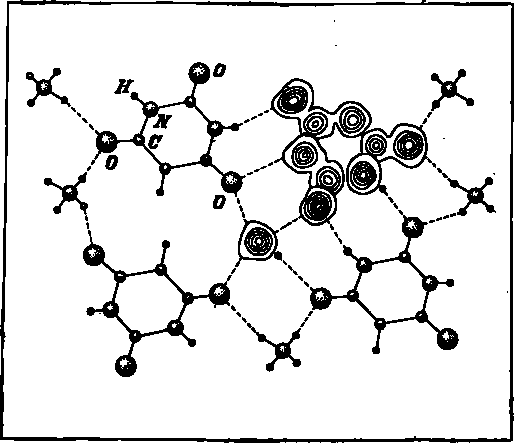
\includegraphics[width=\textwidth]{figures/fig-03-03.pdf}
\caption{Crystal structure of ammonium barbiturate.}
\label{fig-3.3}
\end{figure}
In what form does the physicist (the specialist in $X$-ray diffraction analysis) provide the chemist with informa­tion concerning structure? Some idea of this can be gained by a glance at \figr{fig-3.3}, which shows a very simple structure called ammonium barbiturate. Today, determin­ing the structure of such complexity is child's play. An automatic device gives the structure without any effort on the part of the researcher. The electronic computer can print out the numbers (the values of the coordinates of the atoms) or can produce displays like that of \figr{fig-3.3}. Atoms of different kinds are symbolized by circles of different size. And if the researcher wants the computer to give a picture of electron density, it can do so. Each atom is displayed in the way that geographers portray lines of equal altitude in mountainous regions. But in our case the closed circuits are not lines of equal altitude but curves indicating the electron density at every point. The tip of the ``mountain peak'' is the centre of the atom.

The accompanying diagram is a very minute portion of the contribution that this method has made to science. The success of the method is colossal. To date, the struc­tures of over 15 thousand crystals have been deciphered, and these include several tens of structures of proteins whose molecules consist of many thousands of atoms. 

Determining the structures of complex molecules lays the foundation of biological chemistry and biological physics, two new sciences that have burst into bloom and are expected to give us discoveries of the secrets of life, illness, and death. Despite its sixty-some years of existence, $X$-ray diffraction analysis remains at the forefront of science.

\section{The X-ray Spectrum}

In the preceding section we mentioned the existence of a ``white'' spectrum and monochromatic rays. How can we decipher the nature of the spectrum of hard electromagnetic radiation? And when is it ``white'' and in what cases is it monochromatic?
\begin{figure}[!ht]
\centering
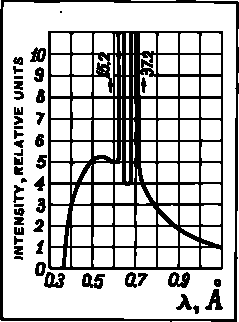
\includegraphics[width=0.4\textwidth]{figures/fig-03-04.pdf}
\caption{The $X$-ray spectrum of molybdenum anode.}
\label{fig-3.4}
\end{figure}

If we diaphragm $X$-rays or gamma rays coming from some source (that is, if we place in their path two screens with small openings) and make the beam impinge on a crystal, then in the most general case we obtain several rays reflected from planes that are in positions that sat­isfy the Bragg-Vulf equation. If we position the crystal so that some plane (yielding a strong reflection) coincides with the axis of rotation of a special instrument (called an \emph{$X$-ray spectrograph}) and then turn the crystal so that the plane comes under the incident ray at a succession of all angles $\theta$, then a component of the spectrum with a definite wavelength will be reflected for each position of the crystal. This reflected wave can be either picked up by an ionization counter or recorded on film. In this way we can create a monochromatic ray of any wavelength of the radiation spectrum and, also, develop a method for exploring the spectrum of any type of radiation.

A typical spectrum of an $X$-ray tube with molybdenum anode is shown in \figr{fig-3.4} (at 35 kilovolts). The con­clusion is almost immediate that there are two reasons for the generation of an $X$-ray spectrum. We see that the observed spectrum is a superposition of sharp peaks on a continuous curve. Of course, the origin of these peaks differs from the origin of the solid curve.

Immediately after the discovery of the diffraction of $X$-rays, a study began of $X$-ray spectra and the following was established. A continuous spectrum is not typical of the material of the anode and depends on the voltage. Its peculiarity is that it breaks off sharply at a certain minimum wavelength. When moving in the direction of long wavelengths, the curve passes its maximum and smoothly falls off without having any apparent endpoint.

By increasing the voltage in the $X$-ray tube, researchers demonstrated that the intensity of the continuous spec­trum grows and the boundary is shifted towards the short waves. And the following very simple equation was estab­lished for the boundary wavelength:
\begin{equation*}%
\lambda_{\textrm{min}} = \frac{12.34}{U}
\end{equation*}
In quantum language, the statement of the rule is simple. The quantity $eU$ is the energy gained by an electron in covering the distance from the cathode to the anode. Naturally, the electron cannot release more energy than this quantity indicates. If it transfers all the energy to generating an $X$-ray quantum $(eU=h\nu)$, then after sub­stituting the constants we obtain the above equation ($\lambda$ is in angstroms and $U$ in kilovolts).

Since we get a continuous spectrum, it follows that the electrons do not necessarily give up all their energy to the generation of $X$-rays. Experiment shows that a large part of the energy of an electron beam is converted into heat. The efficiency of an $X$-ray tube is very low. The anode heats up and it has to be cooled by means of water flowing inside the anode.

Is there a theory that can explain the reason for a continuous spectrum of $X$-rays? Yes, there is. Calculations (which unfortunately we cannot give here) show that from the general laws of the electromagnetic field (from Maxwell's equations) that were discussed in book three of this series, it follows very rigorously that if electrons are decelerated, the result is a continuous spectrum of $X$-rays. Collisions with a solid are not essential at all. If the electrons are decelerated by means of a counter­ field, the result is a continuous emission of $X$-rays without any participation of the anode in the game.

There is yet another way of encountering a continuous $X$-ray spectrum. We recall that a continuous electro­magnetic spectrum is emitted by incandescent bodies. In terrestrial conditions we do not encounter an $X$-ray spectrum of such origin because (compare the formula given on page \pageref{lambdamax}) at the highest possible temperature of an incandescent body (6000 degrees -- since no solid body can stand up to a higher temperature) the wavelength of thermal radiation will be close to half a micrometre. But we must not forget about the existence of plasma. In stellar interiors and in artificial plasma produced here on earth, temperatures in the millions of degrees can be obtained. Then the thermal spectrum of electromagnetic radiation will also include $X$-rays. $X$-rays coming from outer space help resolve intriguing problems of astrophysics.

Now let us touch on the sharp peaks that are superim­posed on the curve of the continuous spectrum.

Just the reverse was proved with respect to these rays, the reverse with respect to the law of the continuous spectrum. The sites of the peaks, that is, their wave­ lengths, are unambiguously determined by the material of the anode. Such emission therefore goes by the name \emph{characteristic}.

Its origin is unbiasedly accounted for by the quantum model of the atom. The electron rays of an $X$-ray tube are capable of penetrating an atom of the anode and knocking out electrons from the very lowest energy levels. As soon as a low level is vacated, that site is filled by an electron more distant from the centre of the atom. Energy is emitted in accordance with the basic quantum law: $E_{m} - E_{n}=hv$. Energy levels are arranged in different ways in different atoms. It is therefore natural that the new spectra will be characteristic spectra.

Since the lines of a characteristic spectrum are the strongest ones, they are used for $X$-ray diffraction analy­sis. It is best to eliminate the continuous spectrum; that is, before making the ray fall on the crystal under inves­tigation, it has to be reflected from the crystal monochro­mator.

Since the spectra of different elements are characteris­tic, a dispersion of the ray into a spectrum may be used for purposes of chemical analysis. It is called \emph{$X$-ray spec­tral analysis}. There is a whole range of fields (for example the study of rare-earth elements) where $X$-ray spectral analysis is absolutely indispensable. The intensities of spectral $X$-ray characteristic lines make it possible to determine to a high degree of accuracy the percentage content of any element in a mixture.

Now a word or two concerning the spectra of gamma rays. In terrestrial conditions, we have to do with gamma rays that originate in radioactive decay (this will be dis­ cussed later on). Radioactive disintegration may or may not be accompanied by the emission of gamma radiation. But no matter what the type of radioactive decay, the spectrum of gamma radiation will be characteristic.

If characteristic $X$-rays appear when an atom falls from a high energy level to a lower level, then gamma rays are produced as a result of a similar transition of the atomic nucleus.

The gamma-ray spectra of radioactive transformations have been thoroughly studied. There are tables in which one can find exact data on the wavelengths of gamma rays generated in alpha- and beta-transformations of one or another radioactive isotope.

\section{Radiography of Materials}

I have time and again had to call attention to the fact that terminology is a weak spot in science. Science develops at such a rate that the meaning of a term changes in the course of a single generation. And at the same time, changes in terminology are associated with altera­tions of what is taken to be accepted. What is more, old books cannot be taken out of circulation, and so the only thing left is to include strict definitions of every term that is employed and to redefine others.

At the present time, when one speaks of $X$-ray diffrac­tion analysis, he has in view the investigation of the atomic structure of crystals. The object of study is a single crystal of the substance.

However, studying structure by means of $X$-rays does not in any way exhaust the problem. Characteristic and information-rich pictures are obtained if radiographs are taken of any materials and not only single crystals. In such cases we ordinarily use the term \emph{radiography}.

If a piece of metal foil is placed in the path of a mono­chromatic $X$-ray beam, a system of concentric circles ap­pears on a flat photographic plate. A radiograph of this type is termed a \emph{Debye crystallogram}. What is its origin?

Most solids consist of tiny crystals oriented at random with respect to one another. When a melt of some sub­stance begins to cool, crystallization sets in simultaneous­ly at a large number of sites. Each minute crystal grows every which way and the growth continues until the crystals meet.
\begin{figure}[!ht]
\centering
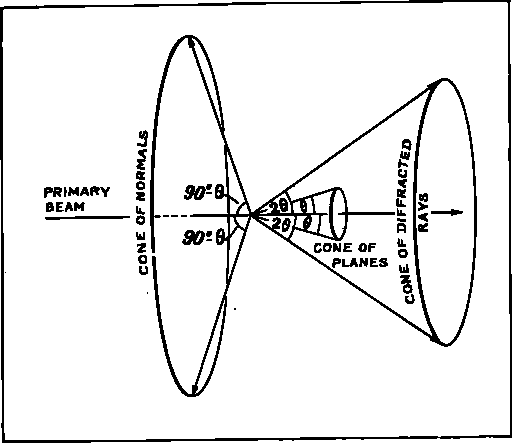
\includegraphics[width=0.8\textwidth]{figures/fig-03-05.pdf}
\caption{Reflections from crystals in solids form a cone.}
\label{fig-3.5}
\end{figure}


Each crystal has the same system of atomic planes; this is because we are dealing with structurally identical crystals. Let us examine one of these systems of planes with interplanar spacing $d$. There are a large number of minute crystals (ordinarily, the linear dimensions of a solid-body crystal is, as to order of magnitude, equal to one ten-thousandth of a centimetre), and among them are those whose planes lie at an angle $\theta$ to the incident ray, which angle satisfies the Bragg-Vulf equation. Each such crystal will leave a spot on a photographic plate. Reflections will be produced by all such minute crystals whose normals to the planes form a cone (\figr{fig-3.5}). If that is so, then the reflected rays will lie in the cone. The intersection of that cone with the photographic plate yields a circle. By measuring the radii of the circles and knowing the distance from the object to the photographic plate, we can find the Bragg angle $\theta$ at once and will then be able to calculate all the interplanar spacings of the substance on the basis of such a radiograph.


Using such a diffraction pattern, we can at once distinguish any amorphous material from crystalline material. Amorphous bodies do not have reflecting planes. Therefore the radiograph will not reveal any system of distinct diffraction rings. There is always some sort of order in the arrangement of molecules of a substance for the simple reason that atoms cannot ``overlap'' in any way. And as calculations show, this results in the radiograph of an amorphous body having one or (rarely) two smeared rings.

However, the rings observed on radiographs yield a good deal of valuable information concerning the struc­ture of materials such as metals, polymers, and natural compounds. If the substance consists of large crystallites, then the diffraction ring will not be continuous and will consist of separate small spots. If the crystallites are not arranged haphazardly but are oriented along an axis or plane, as occurs in wire or sheets of metal, in polymer strands and in vegetable fibres, then the diffraction rings will tell us so immediately. It is easy to see that if we have preferential orientations of crystallites, the reflec­tions from atomic planes will not fill the cone of rays in a continuous fashion. In place of rings, the radiograph reveals arcs. And if the orientation is highly refined, these arcs may degenerate into tiny spots.

Of course, to give a detailed description of the type of structure from the form of radiograph is no easy prob­lem. In this case, too, the method of trial and error plays an essential role. The investigator thinks up models of the structure of materials, calculates patterns of reflec­tions of $X$-rays that should yield the models he has con­cocted and, by comparing calculations and experiment, chooses the proper pattern for the structure of the sub­stance.

In the radiography of materials we distinguish, some­what artificially, between scattering through large and small angles. From the Bragg-Vulf equation given above, it is clear that scattering through large angles occurs if a structural periodicity is observed at small distances (say, \SIrange{3}{10}{\angstrom}). If the reflected (we could say, scattered) $X$-rays yield a diffraction pattern that collects near the primary beam, then this means the structure possesses periodicity at large distances.

In the science of metals we deal mainly with diffrac­tion rings located at large angles, since they consist of crystallites whose atoms form regular lattices with cells having dimensions of the order of units of angstroms.

When the objects of investigation are substances made up of macromolecules, we encounter a very interesting situation. (By the way, macromolecules are found in many natural substances such as cellulose or DNA and also synthetic polymer materials with such familiar names as polyethylene, nylon, capron and so on.) In some cases we obtain radiographs exhibiting rings of large diameter only. In other words, we have to do with the same kind of scattering through large angles as is the case in metals. And at other times, on occasion, we do not find large-diameter rings but rather diffraction rays that only slightly deviate from the primary direction. Finally, there are cases where the substance reveals $X$-ray scattering both through large and small angles.

Small-angle scattering (of course the division into types of small-angle and large-angle scattering is somewhat artificial) is in the range from several minutes to \ang{3} to \ang{4}. Naturally, the smaller the diffraction angle the greater the repeating period of structural elements that produced the diffraction.

Large-angle scattering is due to the order in the loca­tion of atoms inside the crystallites. Small-angle scatter­ing, on the other hand, is connected with the ordered arrangement of rather large formations that are called permolecular. It can even turn out that there is no order at all inside these formations consisting of hundreds and even thousands of atoms. But if such large systems form one-dimensional, two-dimensional or three-dimensional lattices, then small-angle $X$-ray scattering will tell the story. To get a picture of what I mean, imagine a carefully arranged structure made up of bags of potatoes. It is extremely interesting, and probably there is pro­found meaning in the fact that we encounter just such a ``baggy'' order in a very large number of biological sys­tems. For example, the long molecules that make up muscle tissue are arranged very accurately, like a package of round pencils. As small-angle $X$-ray scattering shows, we find just such extraordinarily high order in cell mem­branes, in such protein systems as viruses, and so on.

There is an interesting theorem in the theory of diffrac­tion. I will not try to prove it but I'm sure it will appear natural to the reader. It can be rigorously demonstrated that the type of diffraction pattern remains the same if in the object that produces the diffraction we inter­change the apertures and opaque places. This theorem sometimes makes the research worker miserable. It is when $X$-ray scattering can be caused either by pores within the substance or by extraneous inclusions. The study of pores -- their dimensions, shape, and quantity per unit volume -- is of great practical interest. The colouring of synthetic fibres depends to a very large extent on these peculiarities in their structure. It is easy to see that an uneven distribution of pores will result in an uneven colouring and a final unpleasant fabric.

From what has been said it is now sufficiently obvious that radiography of materials is not only a method of studying substances but also a method of technical con­trol in a great variety of industries.
%
%%\newpage
%\begin{center}
%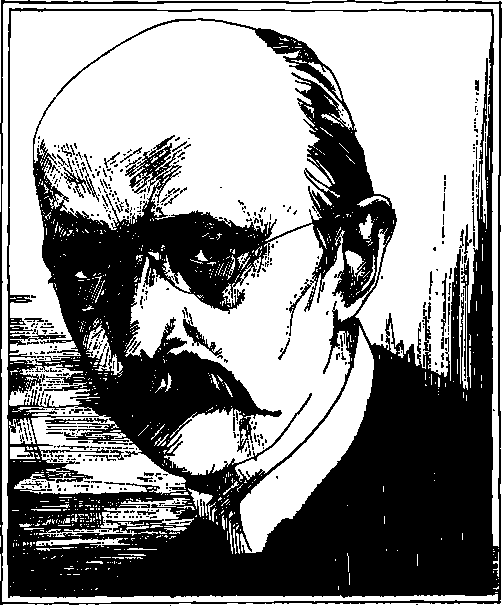
\includegraphics[width=\textwidth]{figures/planck.pdf}
%\end{center}
%{\small \textsf{\hlred{Max Planck [1858-1947]}} -- \textsf{\footnotesize outstanding German scientist who laid the foundations of quantum theory. In an attempt to find a mathematical expression for a proper description of the spectral distribution of the emission of an ideal black body Planck demonstrated that such a formula could be obtained by introducing a ``quantum of action''. Planck assumed that a body emits energy in parcels, equal to the product of a constant (which later was named after him) by the frequency of the light.}}



